\section{Mathematical Background}\label{sec:math-background}
To understand the following chapters in the thesis, we need a brief introduction in complex analysis and multivalued functions. The following mathematical introduction is based on the book \textit{Introduction to Complex Analysis} by H.~A.~Priestley~\cite{ComplexAna:Intro}.

A complex number $z \in \Complex$ is specified by a two real numbers $x$ and $y$ as $z = x+y\iunit$, with $\iunit$ as the imaginary unit, which is defined as a solution of $\iunit^2 = -1$. The two real numbers are called the real part $x = \Re(z)$ and the imaginary part $y = \Im(z)$ of $z$. It is convenient to represent complex numbers as points in a $\Real^2$ plane, which is called \textbf{complex plane}. We identify $z = x+y\iunit$ as $(x,y) \in \Real^2$ in the complex plane. It is sometimes useful to represent complex numbers by polar coordinates and write $x = r\cos@@{\phi}$ and $y = r\sin@@{\phi}$, with $r \geq 0$ and $\phi \in \Real$. Since $\cos@@{\phi}+\sin@@{\phi}\iunit$ can be written as $\expe^{\iunit\phi}$, we write $z = x+y\iunit$ in polar coordinates as $z = r\expe^{\iunit\phi}$. The angle $\phi$ is often called the \textbf{phase} (or argument) of $z$ and $r$ is the absolute value of $z$. Similar to $\Re(z)$ for the real part and $\Im(z)$ for the imaginary part of $z$, we can access $r = |z|$ and $\phi = \ph@{z}$.\footnote{Note that the phase of $z$ is often called the \textbf{argument} of $z$. Therefore, in CAS the phase function is often the \texttt{argument} function.}

\begin{figure}[ht]
    \centering
    \subfloat[Four color phase mapping.]{%
        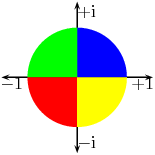
\includegraphics[width=0.28\textwidth]{dlmfColorMap.png}
        \label{fig:four-color}%
    }
    \hspace{0.4cm}
    \subfloat[Continues phase mapping in \DLMF.]{%
        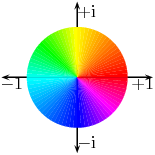
\includegraphics[width=0.28\textwidth]{dlmfColorMapCont.png}
        \label{fig:cont-color}%
    }
    \hspace{0.4cm}
    \subfloat[Continues phase mapping in \Maple.]{%
        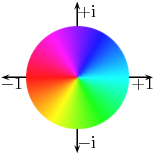
\includegraphics[width=0.28\textwidth]{mapleColorMap.png}
        \label{fig:maple-color}%
    }
    \caption{Three different domain coloring methods. Mappings~\protect\subref{fig:four-color} and \protect\subref{fig:cont-color} used in the \DLMF{} (Source: \DLMF{~}\cite{NIST:DLMF} in help page, \textit{About Color Map}). Mapping~\protect\subref{fig:maple-color} is the default coloring map in \Maple.}
    \label{fig:domain-coloring}
\end{figure}

Since the same basic arithmetical rules apply in $\Complex$ as in $\Real$, we will not introduce all arithmetical rules for complex numbers here. However, another interesting part are plots of complex functions. Consider a function $f: \Complex \mapsto \Complex$. This can be considered as $f: \Real^2 \mapsto \Real^2$, which shows us four real dimensions that need to be displayed in a three-dimensional space. The most common solution to plot those four dimensions is called domain coloring. With this technique, each value in the complex plane is represented by a color. There is no standard method to map complex values to colors. A simple method is to map a unique color for each of the quadrants in the complex plane (used in the DLMF). Another variation are continues phase mappings, which use color wheels. In those cases, $\phi$ represents the hue and optionally $r$ defines the intensity of the hue. The second variation is mostly used in \gls{cas}, but there is no standard for the orientation of the color wheel. Figure~\ref{fig:domain-coloring} draws three different examples.

This thesis mostly focus on the \gls{cas} \Maple, therefore all of the following complex plots use the default color map in \Maple{~}\ref{fig:maple-color}.

A three-dimensional plot of a complex function, such as $f$ from above, usually maps the real and imaginary part of the variable to the $x$ and $y$ axes, while the height is defined by the absolute value of the complex variable $|z|$. Figure~\ref{fig:cylinderU} demonstrates a complex plot of the parabolic cylinder function $\ParabolicU@{a}{z}$~\cite[(12.2i)]{NIST:DLMF} in \Maple. 

\begin{figure}[ht]
	\centering
	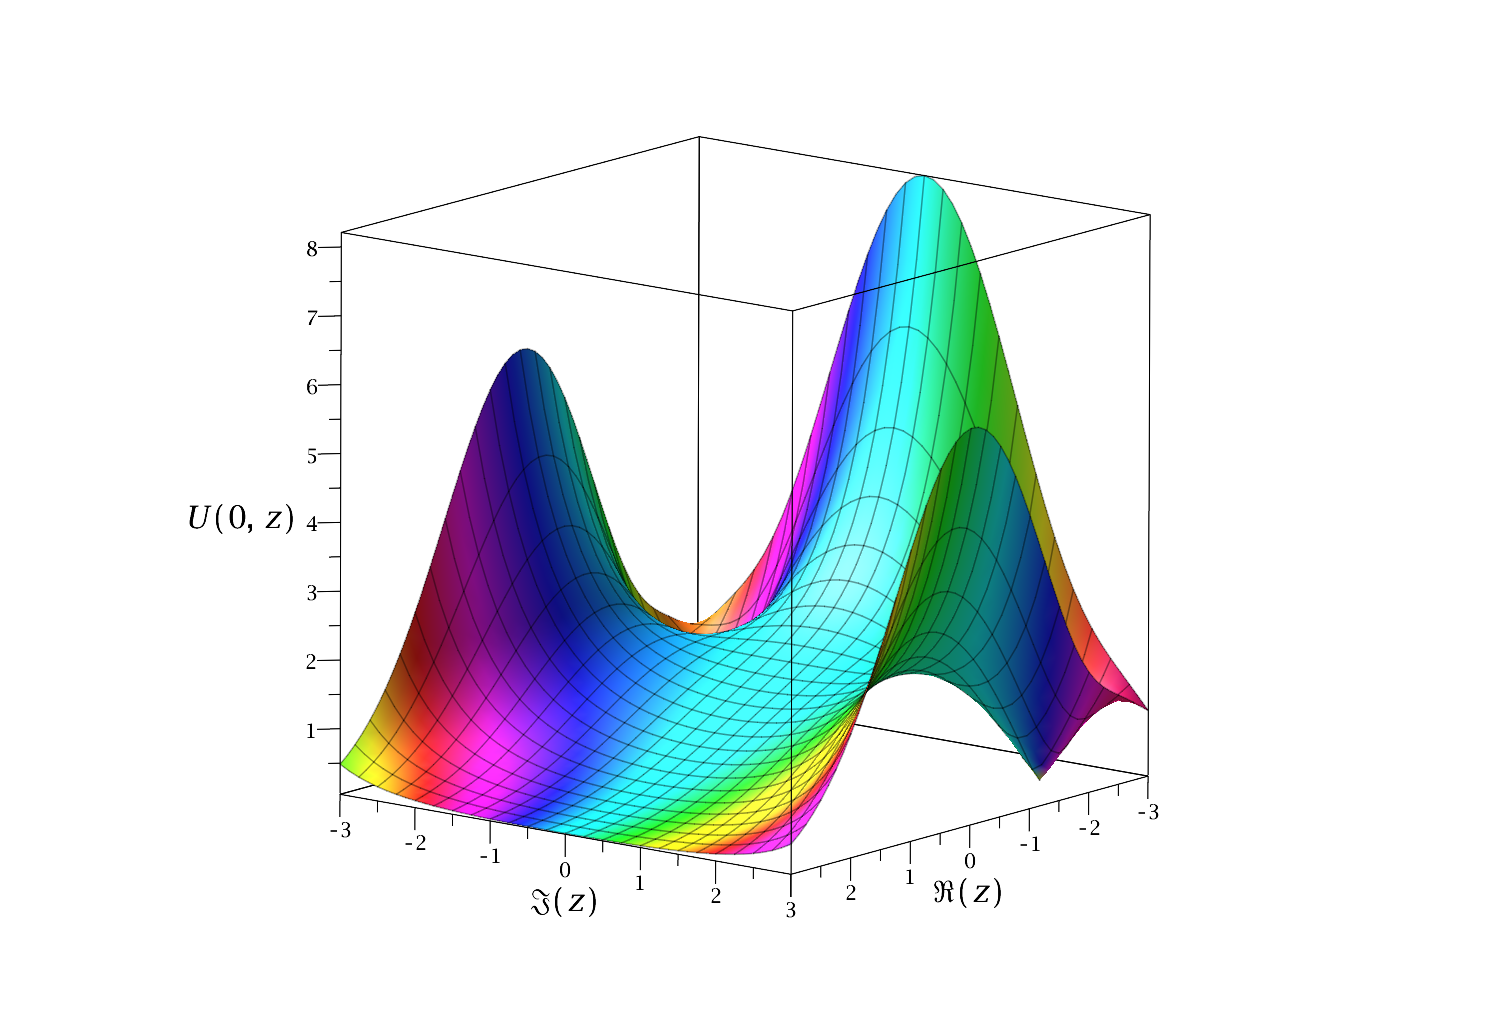
\includegraphics[width=0.8\textwidth]{cylinderUPlot.png}
	\caption{A 3-dimensional complex plot of the parabolic cylinder function $\ParabolicU@{a}{z}$ at $a=0$ plotted by \Maple.~\cite[(12.2i)]{NIST:DLMF}}
	\label{fig:cylinderU}
\end{figure}

Another way to plot such complex functions is to plot the real and imaginary parts of the solution separately. Figure~\ref{fig:cylinderUSplit} illustrates this plotting method for the parabolic cylinder function again. 

Note that for real function plots, such separate plots for the imaginary and real values of a complex function, will use a color map as well. In that case, the color map is just an adornment and has nothing to do with complex color maps. Figure~\ref{fig:cylinderUSplit} illustrates the separate plots for real and imaginary values for the parabolic cylinder function again.

\begin{figure}[!htp]
    \centering
    \subfloat[Plot of the real value of $\ParabolicU@{0}{z}$.]{%
        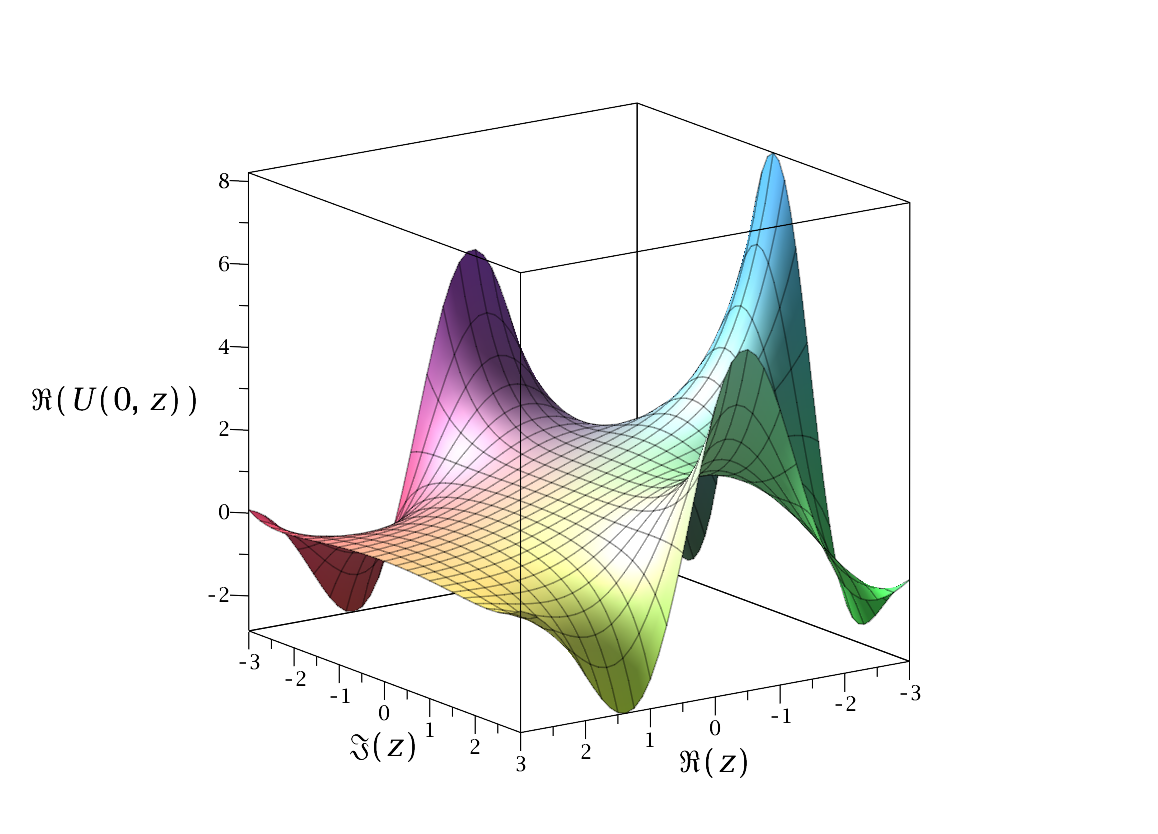
\includegraphics[width=0.8\textwidth]{cylinderURe.png}
        \label{fig:cylinderURe}%
    }
    \vspace{-0.1cm}
    \subfloat[Plot of the imaginary value of $\ParabolicU@{0}{z}$.]{%
        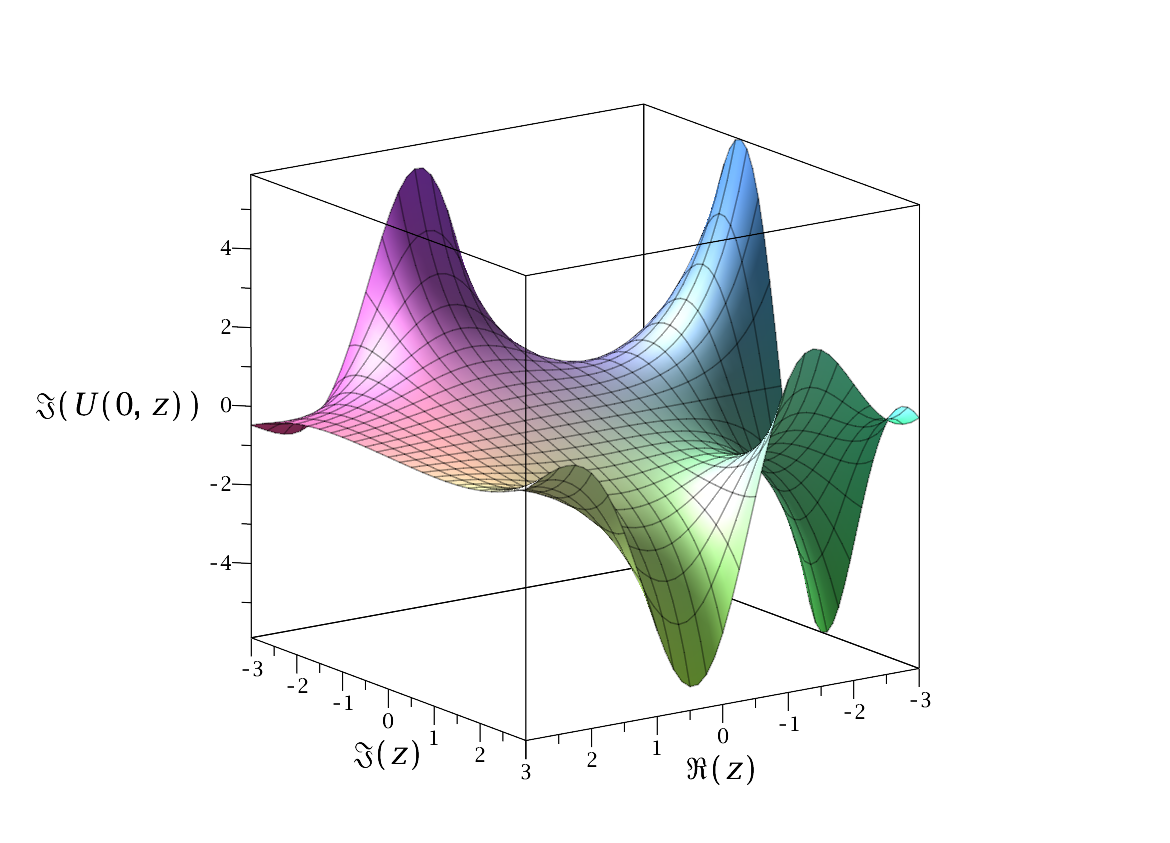
\includegraphics[width=0.8\textwidth]{cylinderUIm.png}
        \label{fig:cylinderUIm}%
    }
    \caption{Separately plot of the real~\protect\subref{fig:cylinderURe} and imaginary~\protect\subref{fig:cylinderUIm} part of the parabolic cylinder function $\ParabolicU@{a}{z}$ at $a=0$.}
    \label{fig:cylinderUSplit}
\end{figure}

\subsection{Multivalued Functions}
The following definitions for multivalued functions are based on \textit{Complex Variables}~\cite{ComplexVariables} by M.~J.~Ablowitz and A.~S.~Fokas.

Unlike a typical\footnote{In lack of a better word to distinguish single-valued and multivalued functions, we call single-valued functions here typical functions, because these functions are best known.} function, multivalued functions associate not only one output to any particular input, but a whole set of output values. A real-valued example is the square root function, which associates for each positive real number two real square roots. For example\footnote{Note that the radical sign $\sqrt{}$\ is defined for the principal square roots, which are the unique non-negative square roots. Therefore, $\sqrt{4}$ is always $2$, and not $-2$. However, the solutions of the square root of a positive number $a$ are $\left\{+\sqrt{a},-\sqrt{a}\right\}$.}, the solution of $4^{\frac{1}{2}}$ is $\{+2,-2\}$.

Consider now the natural logarithm with complex arguments and $z = r\expe^{\iunit\phi}$ in polar coordinates. Since it is the natural logarithm, $\ln@{z} = \ln@{r} + \iunit\phi$ and the imaginary part is just $\phi$. Let $r = 1$, so that $z$ is on the unit circle for all $\phi$. Let be $z_1$ the complex number for $\phi = 0$ and $z_2$ the complex number for $\phi = 2\cpi$. Obviously $z_1 = z_2$ but $\ln@{z_1} \neq \ln@{z_2}$. Therefore, the natural logarithm is also multivalued and has an infinite number of solutions for $\ln@{z}$. 

The center of the circle we choose (in that case the origin) is called branch point.

\begin{definition}[Branch Point]
A point $p$ is a \textbf{branch point} if the multivalued function $w(z)$ is discontinuous upon traversing an arbitrarily small circuit around $p$.
\end{definition}

The complex square root function has also a branch point in the origin. Consider
\begin{equation}
\sqrt{z} = \sqrt{r} \expe^{\frac{\iunit\phi}{2}},\quad \text{with } r \geq 0, \phi \in \Real.
\end{equation}
Indeed, at $\phi = 2\cpi$, the square root of $z$ is $\sqrt{r}\expe^{\iunit\cpi} = -\sqrt{r}$, but at $\phi = 0$ it is $\sqrt{r}$. Because $r$ was arbitrary, the origin is also a branch point of the complex square root function. Another branch point is $z = \infty$.

There exist two approaches to analytically study multivalued functions. One approach is to express the multivalued function as a single-valued function.

\subsubsection{Branch Cuts}\label{subsec:branch-cuts}
Consider a multivalued function in a restricted region and choose for every argument a value, such that the resulting function in the region is continues and single-valued. This regional function of the multivalued function is called \textbf{branch} of the multivalued function. 

Consider the complex square root function again. If we cut out the region between both branch points, namely $(0, \infty)$, the function is continues and single-valued. This region is one branch of the function and the cut region $(0, \infty)$ is called \textbf{branch cut}. Another branch of the function can be reached by further increasing $\phi$, such that $\phi \in [2\cpi, 4\cpi)$. At $\phi = 4\cpi$ the square root function returns the same result as for $\phi=0$. Therefore, $\phi \in [4\cpi, 6\cpi)$ is again on the first branch. We can define a branch cut for the complex logarithm as well. As already mentioned, the complex logarithm has an infinite number of branches. Each of these branches can be reached by increasing or decreasing $\phi$ with a multiple of $2\cpi$. Consider $\phi+n2\cpi$ with an integer number $n$. The branch for $n=0$ is called the \textbf{principal branch}.

Defining branch cuts to allow analytic computations on the principal branches is a common task for \gls{cas}~\cite{Maple:Cuts}. Unfortunately, the position of the branch cuts is not well-defined. Indeed, consider $\phi \in [-\cpi,\cpi)$ instead of $\phi \in [0,2\cpi)$ and define the branch cut at $(-\infty, 0)$; than the branch is also continues and single-valued. 

In general a branch cut is a curve which ends can be possibly open, half-open or closed. A branch cut can be also defined in a more complicated shape (e.g. spirals). Most of the multivalued functions have standard, convenient positions for the branch cuts, which are commonly accepted. The branch cut at $(-\infty, 0]$ for the complex square root function is one of those standard positions. However, the positions can vary from system to system~\cite{Branches:acot}.

Figure~\ref{fig:sqrtBranch} draws the principal branch of the imaginary part of the complex square root function in \Maple.
 
\begin{figure}[ht]
	\centering
	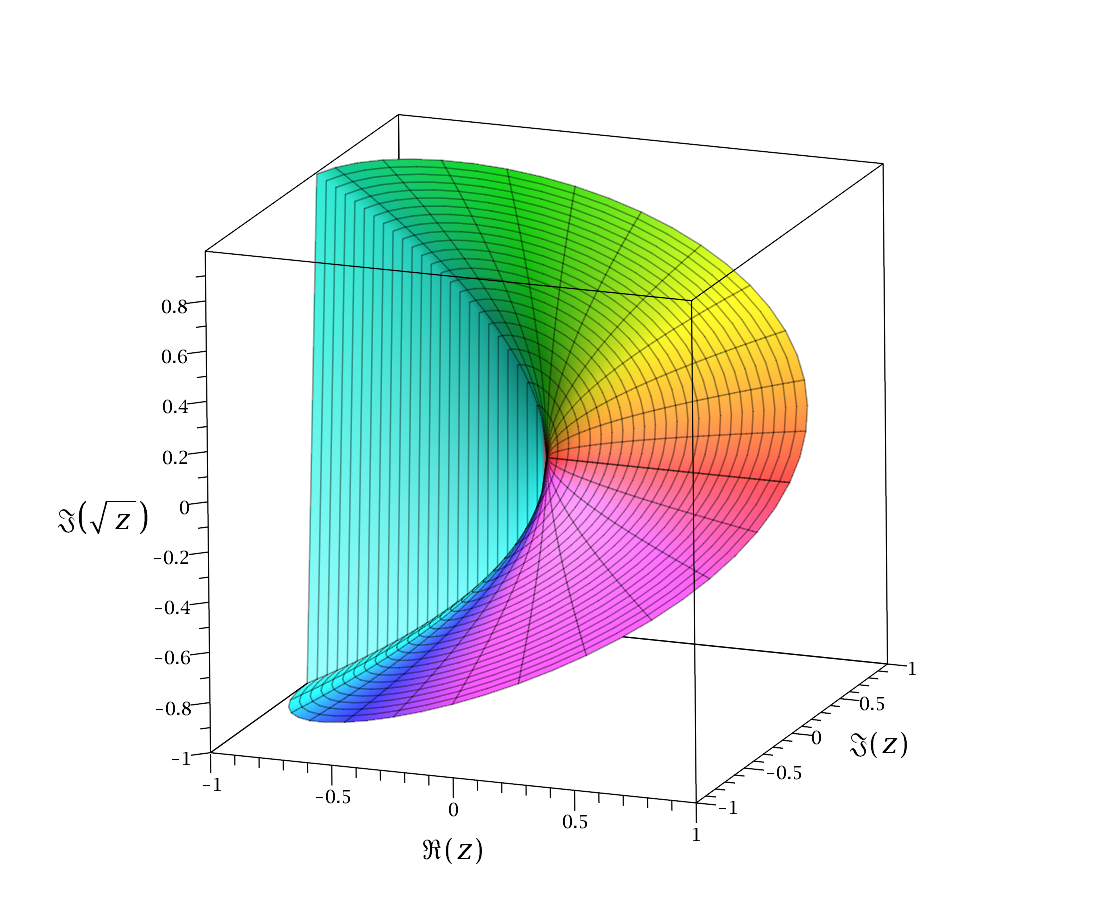
\includegraphics[width=0.65\textwidth]{sqrtBranch.png}
	\caption{The imaginary part of the complex square root function with a branch cut at $(-\infty, 0)$. The resulted function is continues and single-valued for $\phi \in (-\cpi, \cpi)$.}
	\label{fig:sqrtBranch}
\end{figure}

The plot of the principal branch for the complex logarithm looks similar. The branch cut for the logarithm is in \Maple{} defined at $(-\infty,0)$. Figure~\ref{fig:lnBranch} illustrates the principal branch of the imaginary part of the logarithm.

\begin{figure}[H]
	\centering
	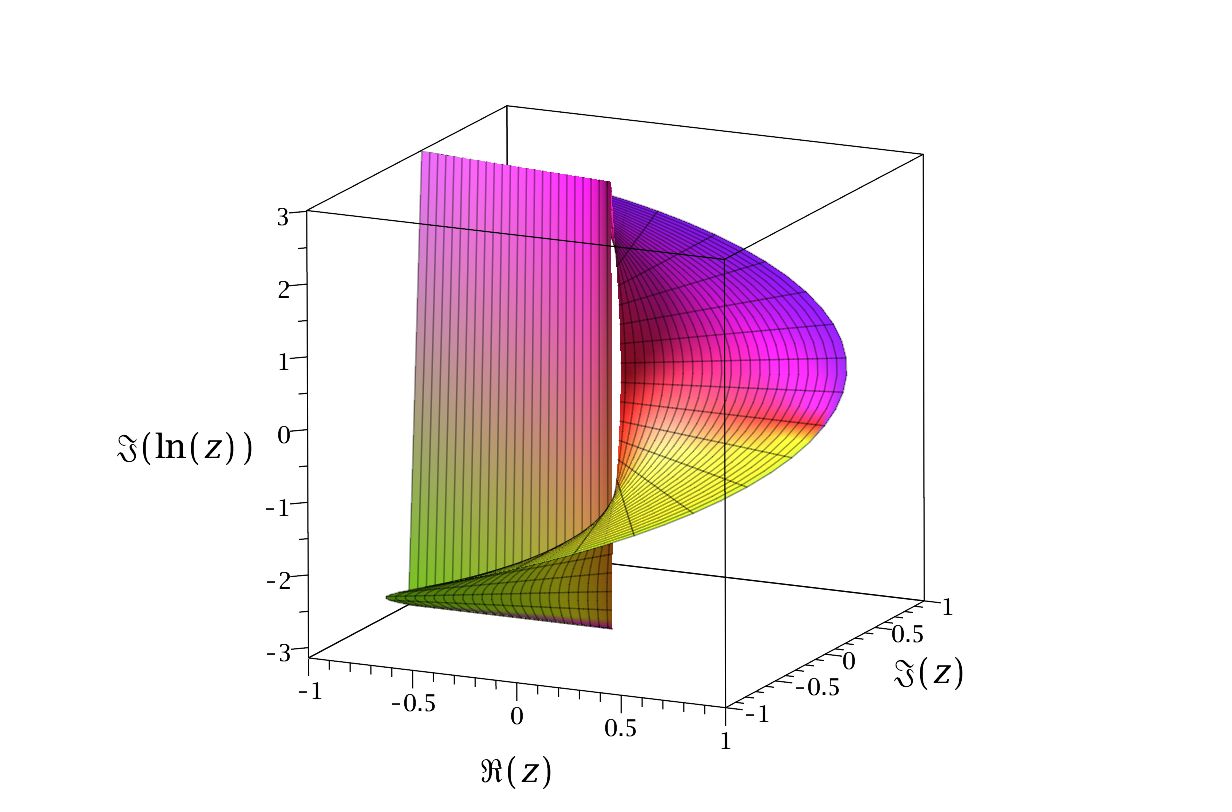
\includegraphics[width=0.75\textwidth]{lnBranch.png}
	\caption{The imaginary part of the complex logarithm with a branch cut at $(-\infty, 0]$. The resulted function is continues and single-valued for $\phi \in (-\cpi, \cpi)$.}
	\label{fig:lnBranch}
\end{figure}

Note that in complex plots, a branch cut can also be located in the color map, we were talking about above. In the next example, we use the notation $\pm 0$ to come arbitrarily close to the branch cut from the \textit{upper} and \textit{lower} side. We presume the one-side limits is a well known notation and define
\begin{align}
-0 &:= \underset{x\nearrow 0}{\lim}x,\\
+0 &:= \underset{x\searrow 0}{\lim}x.
\end{align}

The natural logarithm $\ln@{z}$ has a branch cut at $(-\infty,0]$. We have the following values for the \textit{upper side} and \textit{lower side} of the branch cut at $\ln@{-1}$
\begin{align}
\ln@{-1+\iunit 0} &=\hphantom{-}\iunit \cpi,\label{eq:ln-up}\\
\ln@{-1-\iunit 0} &= -\iunit \cpi.\label{eq:ln-down}
\end{align}

Figure~\ref{fig:ln-compl-comp} shows two plots of the natural logarithm. The value of (\ref{eq:ln-up}) is represented by a shade of purple and (\ref{eq:ln-down}) is represented by a shade of green, with \Maple's continues phase color map from figure~\ref{fig:maple-color}. The branch cut can be seen by the changing of the color from purple directly to green on $(-\infty,0]$. The colors are counterparts of each other in the used color map.

\begin{figure}[!htp]
    \centering
    \subfloat[The complex plot for the natural logarithm $\ln@{z}$. The values of $\ln@{z}$ are visualized by colors. The coloring method is the continues phase mapping from \Maple.]{%
        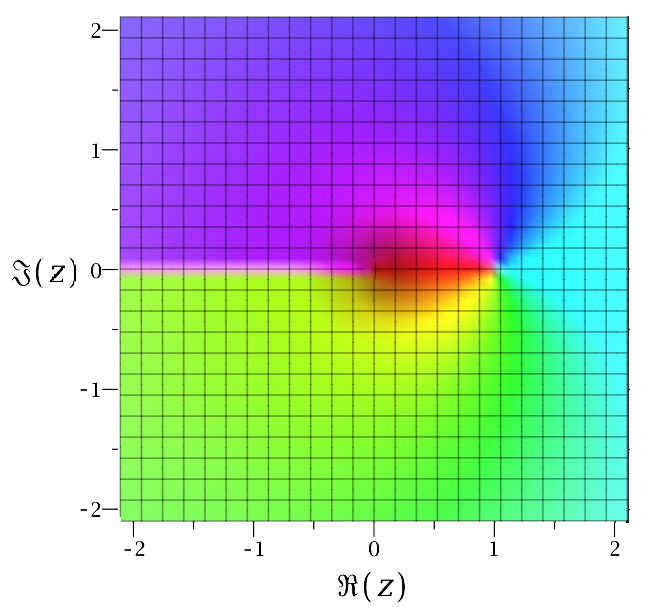
\includegraphics[width=0.4\textwidth]{lnComp1.png}
        \label{fig:ln-color}%
    }
    \hspace{0.5cm}
    \subfloat[The complex plot for the natural logarithm $\ln@{z}$. The height is the absolute value. The coloring method is the continues phase mapping from \Maple.]{%
        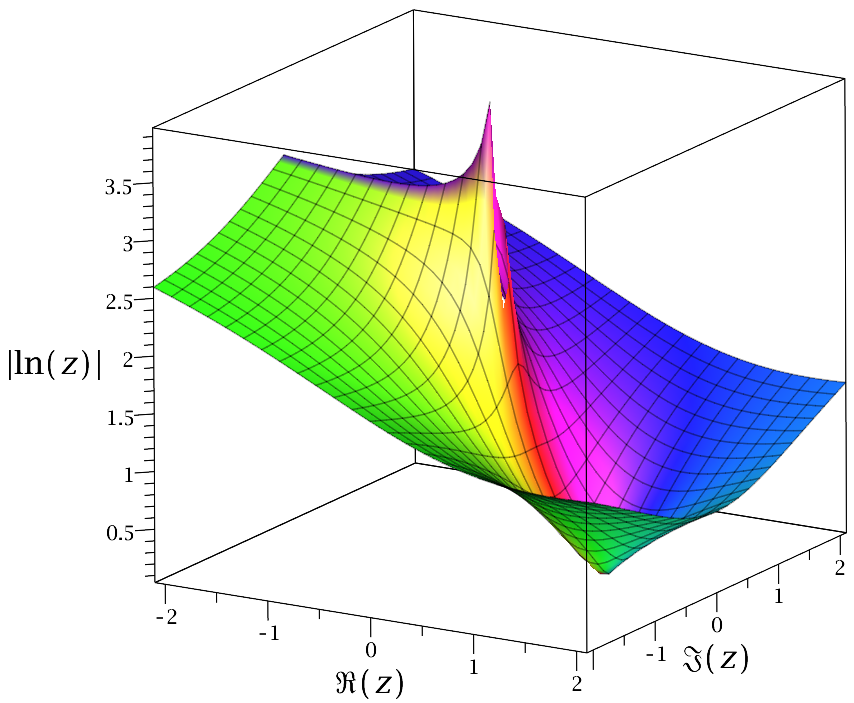
\includegraphics[width=0.47\textwidth]{lnComp2.png}
        \label{fig:ln-compl}%
    }
    \caption{The complex plot of the natural logarithm $\ln@{z}$. Figure~\protect\subref{fig:ln-color} plots only the colors of $\ln@{z}$. The coloring method is \Maple's continues phase mapping from figure~\protect\ref{fig:maple-color}. The branch cut of $\ln@{z}$ is at $(-\infty,0)$ and the values $\ln@{1+\iunit 0} = \iunit \cpi$ (which is mapped to purple), while $\ln@{1-\iunit 0} = -\iunit \cpi$ (which is represented by green).}
    \label{fig:ln-compl-comp}
\end{figure}

An alternative representation for multivalued functions to branch cuts are Riemann surfaces.

\subsubsection{Riemann Surfaces}
Assume we would not cut the multivalued functions and allow multiple values for a particular input. For example, if we allow $\phi$ to constantly increase in the complex logarithm function, we end up in helix structure as plotted in figure~\ref{fig:lnRiemann}. This representation of a multivalued function is called the Riemann surface. Technically, a Riemann surface is a one-dimensional complex manifold.

\begin{figure}[!ht]
	\centering
	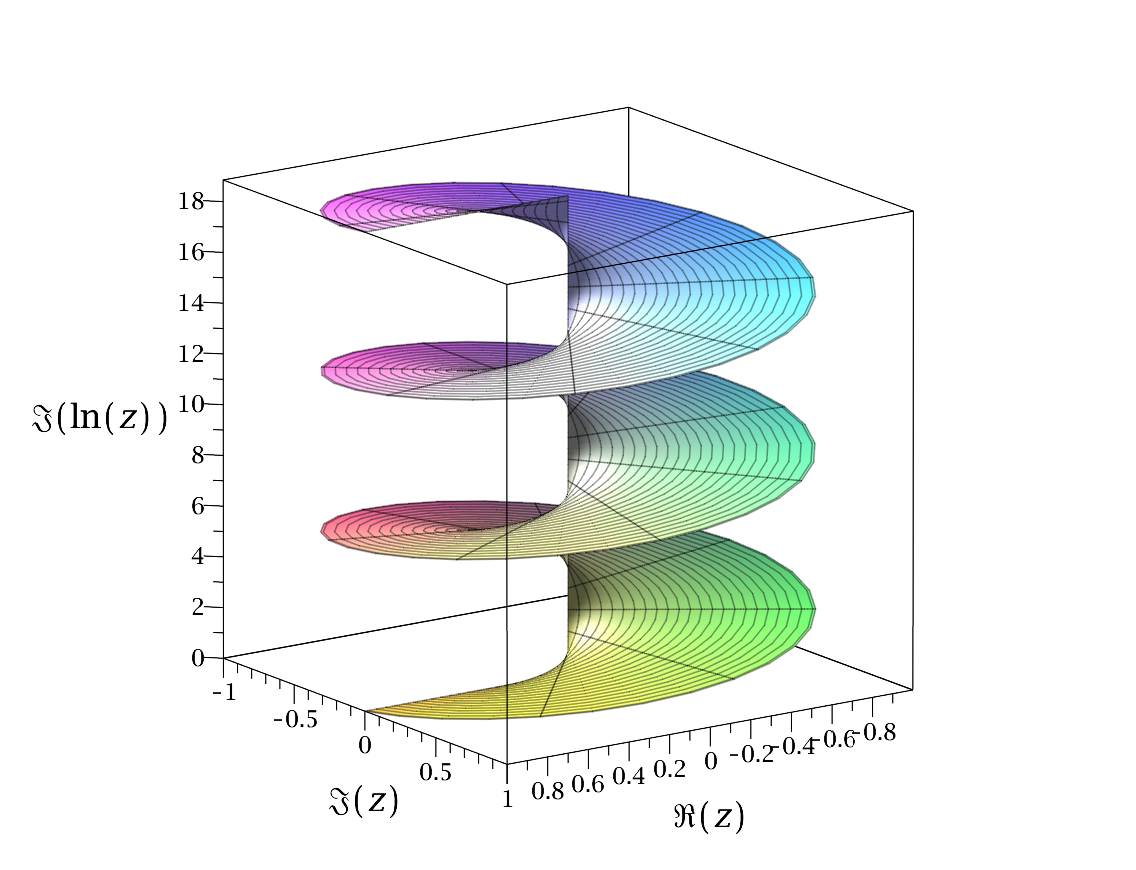
\includegraphics[width=0.8\textwidth]{lnRiemann.png}
	\caption{The Riemann surface of the imaginary part of the natural logarithm.}
	\label{fig:lnRiemann}
\end{figure}

In the Riemann surface of logarithm in figure~\ref{fig:lnRiemann} we can see the multiple branches of the function. If we use the same method for the square root function, we get figure~\ref{fig:sqrtRiemann}, where we can see that the square root function has only two branches.

\begin{figure}[!ht]
	\centering
	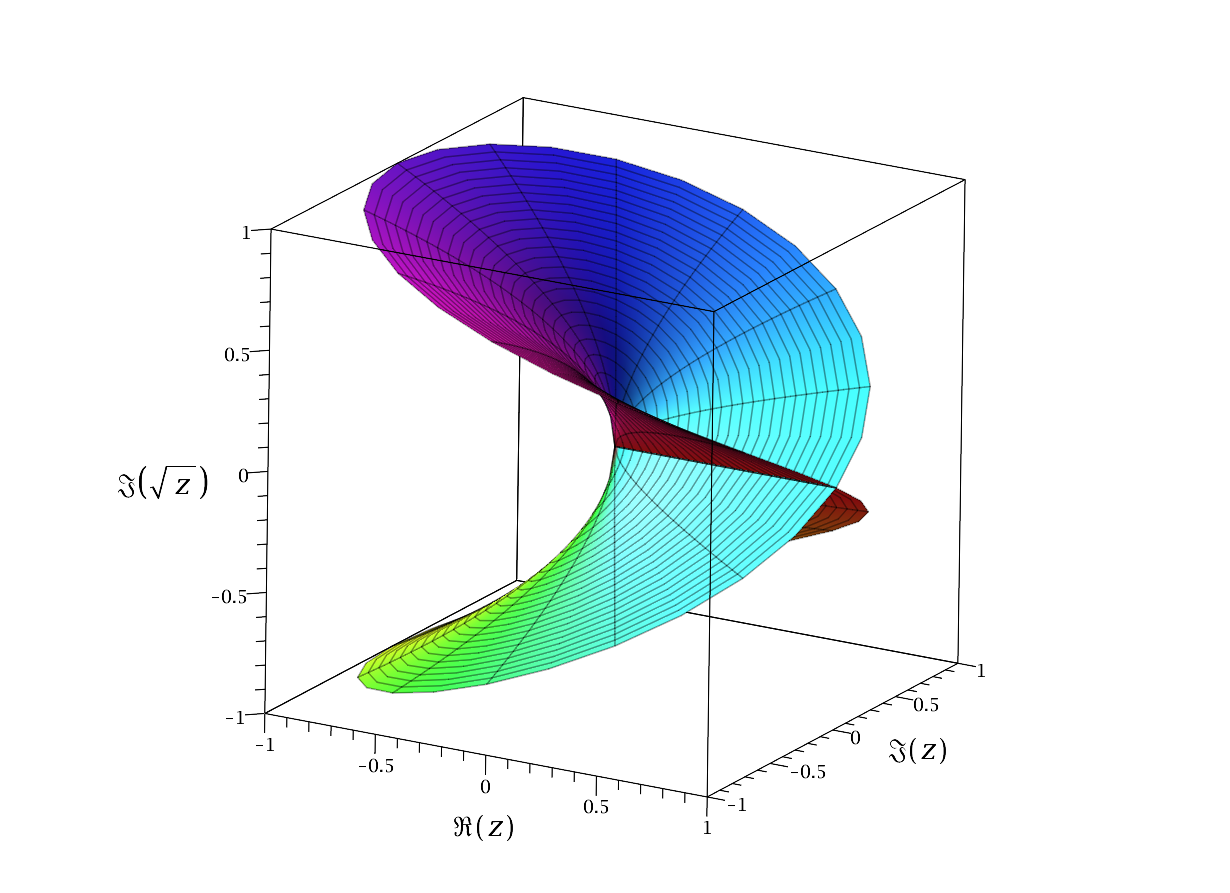
\includegraphics[width=0.9\textwidth]{sqrtRiemann.png}
	\caption{The Riemann surface of the imaginary part of the square root function.}
	\label{fig:sqrtRiemann}
\end{figure}

\subsection{Elementary \& Special Functions}\label{subsec:special-functions}
A function is called \textbf{elementary} if it can be constructed using only a finite combination of constant functions, field operations, and algebraic, trigonometric, exponential, and logarithmic functions together with their inverses~\cites{Elementary:1}[145]{Elementary:2}.

Unlike elementary functions, special functions cannot be listed easily. They are mostly solutions of differential equations or integrals of elementary functions. Almost all of them have established names and notations. Many of them are complex and some are also multivalued. Besides that, special functions are highly related to each other. Therefore, most special functions can be expressed by other special functions. However, there is no general formal definition, but there are lists and mathematical compendia collecting functions which are commonly accepted as special. 

For example, in 1964 Milton Abramowitz and Irene A. Stegun published the \textit{Handbook of Mathematical Functions with Formulas, Graphs, and Mathematical Tables}~\cite{AbramowitzStegun} at \gls{nist}\footnote{In 1988 the \textit{National Bureau of Standards} (NBS) was renamed to the \textit{National Instutute of Standards and Technology} (NIST).}. The handbook became the most comprehensive source of information on special functions. Therefore, the \gls{nist} has published a new version called \textit{NIST Handbook of Mathematical Function}~\cite{NIST:Handbook} in 2010 to replace the predecessor.

Because there is no formal definition for special functions, some problems appear for our translator project. For example the \textit{Encyclop\ae{dia} Britannica} wrote:
\begin{myQuote}{Encyclop\ae{dia} Britannica - Special function~\cite{SpecialFunctions:britannica}}
	Special function, any of a class of mathematical functions that arise in the solution of various classical problems of physics. [...] Different scientists might not completely agree on which functions are to be included among the special functions, although there would certainly be very substantial overlap.
\end{myQuote}

In \textit{Special Functions}~\cite{SF:Book}, G.~E.~Andrews~et~al. wrote in the preface:
\begin{myQuote}{Special Functions - Preface~\cite{SF:Book}}
Paul Tur\'an once remarked that special functions would be more appropriately labeled "useful functions".
\end{myQuote}

Our reference for special functions in this thesis will be the \textit{NIST Handbook of Mathematical Function} and its digital counterpart the \gls{dlmf}~\cite{NIST:DLMF}. See the later section~\ref{sec:dlmf} for a more detailed explanation. 

Since most of the special functions represent solutions for other mathematical expressions, they were intensively studied - mostly in applied mathematics. In the past, huge tables of values were used for calculations~\cite{Tables}. Therefore, the book by Abramowitz and Stegun also contains tables with values for several special functions~\cite{AbramowitzStegun}. Obviously, computations of special functions with \gls{cas} were desired. Therefore, \gls{cas} support numerous of special functions. However, all \gls{cas} contain its own ever growing lists of them. Sometimes they use the same definitions, domains and position of branch cuts as defined the handbooks, sometimes not. A translator needs to pay attention to those differences as well. Otherwise the translation process could produce unexpected effects. One of these effects can be produced by different positions of branch cuts in the systems. The next section will give some examples and explanations of these problems.

\subsection{Problems of Branch Cuts}\label{subsec:branch-cut-issues}
Obviously, different positions of branch cuts can cause problems, if we transfer a function from one system to the other. Those differences can even appear in well-known elementary functions. For example, the \gls{dlmf} defines the branch cut for the inverse cotangent function~\cite[(4.23.9)]{NIST:DLMF} at $[-\iunit, \iunit]$, while \Maple{} reasonably~\cite{Branches:acot} defines the branch cut at $(-\infty\iunit, -\iunit]$ and $[\iunit, \infty\iunit)$. Figure~\ref{fig:acot} illustrates the problem. A scientist, who is familiar with the definition for the branch cut by the \gls{dlmf} would assume an output such as in figure~\ref{fig:acotCont}, but get an output such as in figure~\ref{fig:acotJump} in \Maple.

\begin{figure}[!ht]
    \centering
    \subfloat[Plot of the arccotangent function with the branch cut defined by \DLMF.]{%
        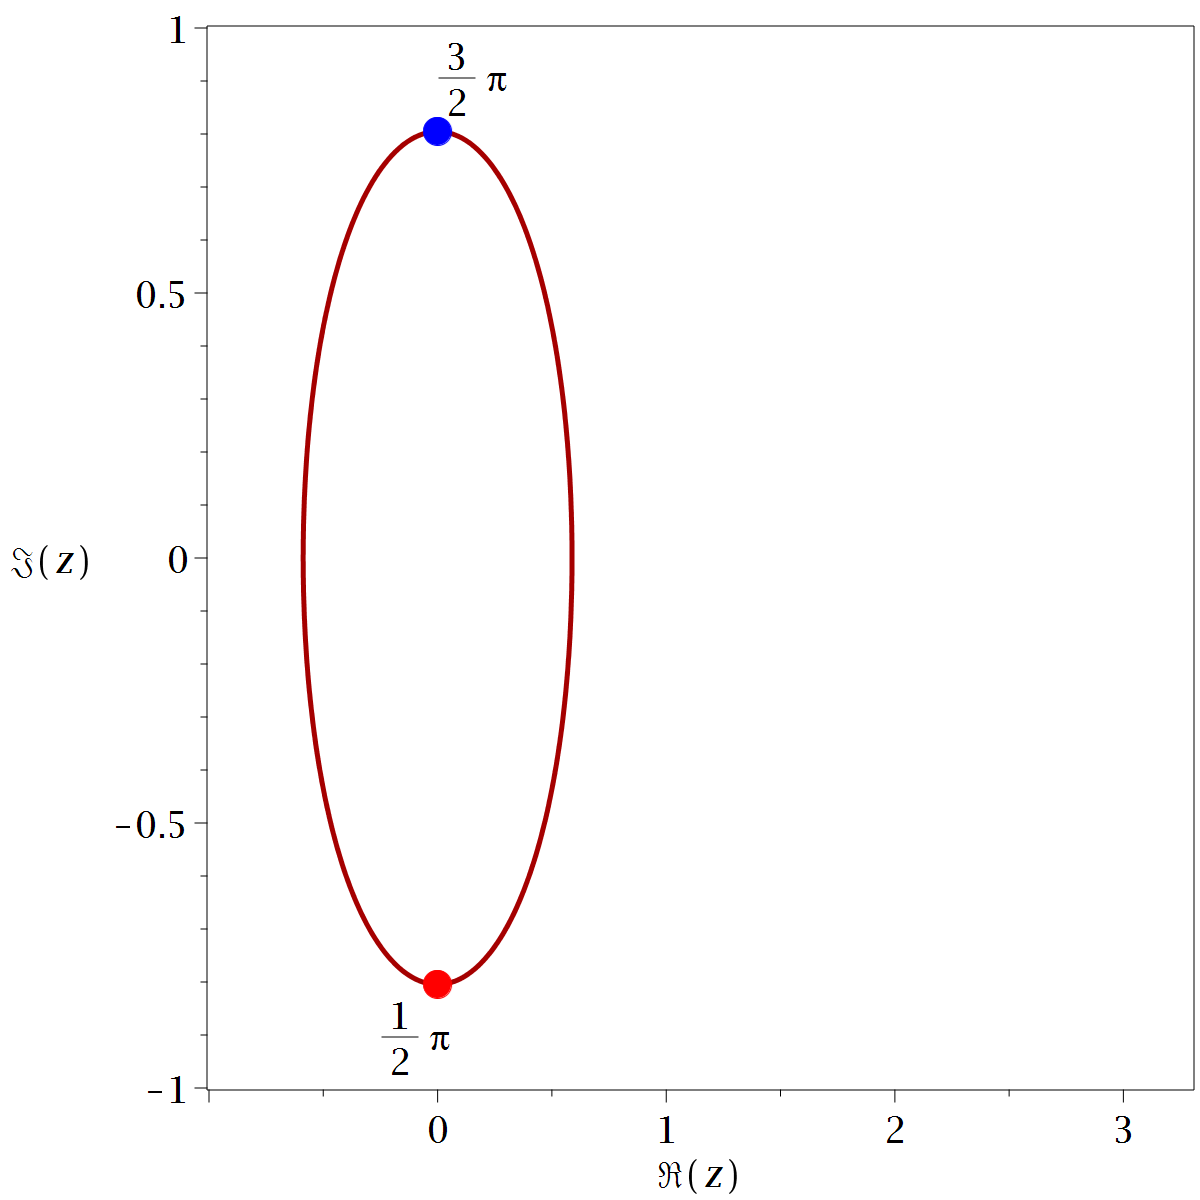
\includegraphics[width=0.45\textwidth]{acotCont.png}
        \label{fig:acotCont}%
    }
    \hspace{0.2cm}
    \subfloat[Plot of the arccotangent function with the branch cut defined by \Maple.]{%
        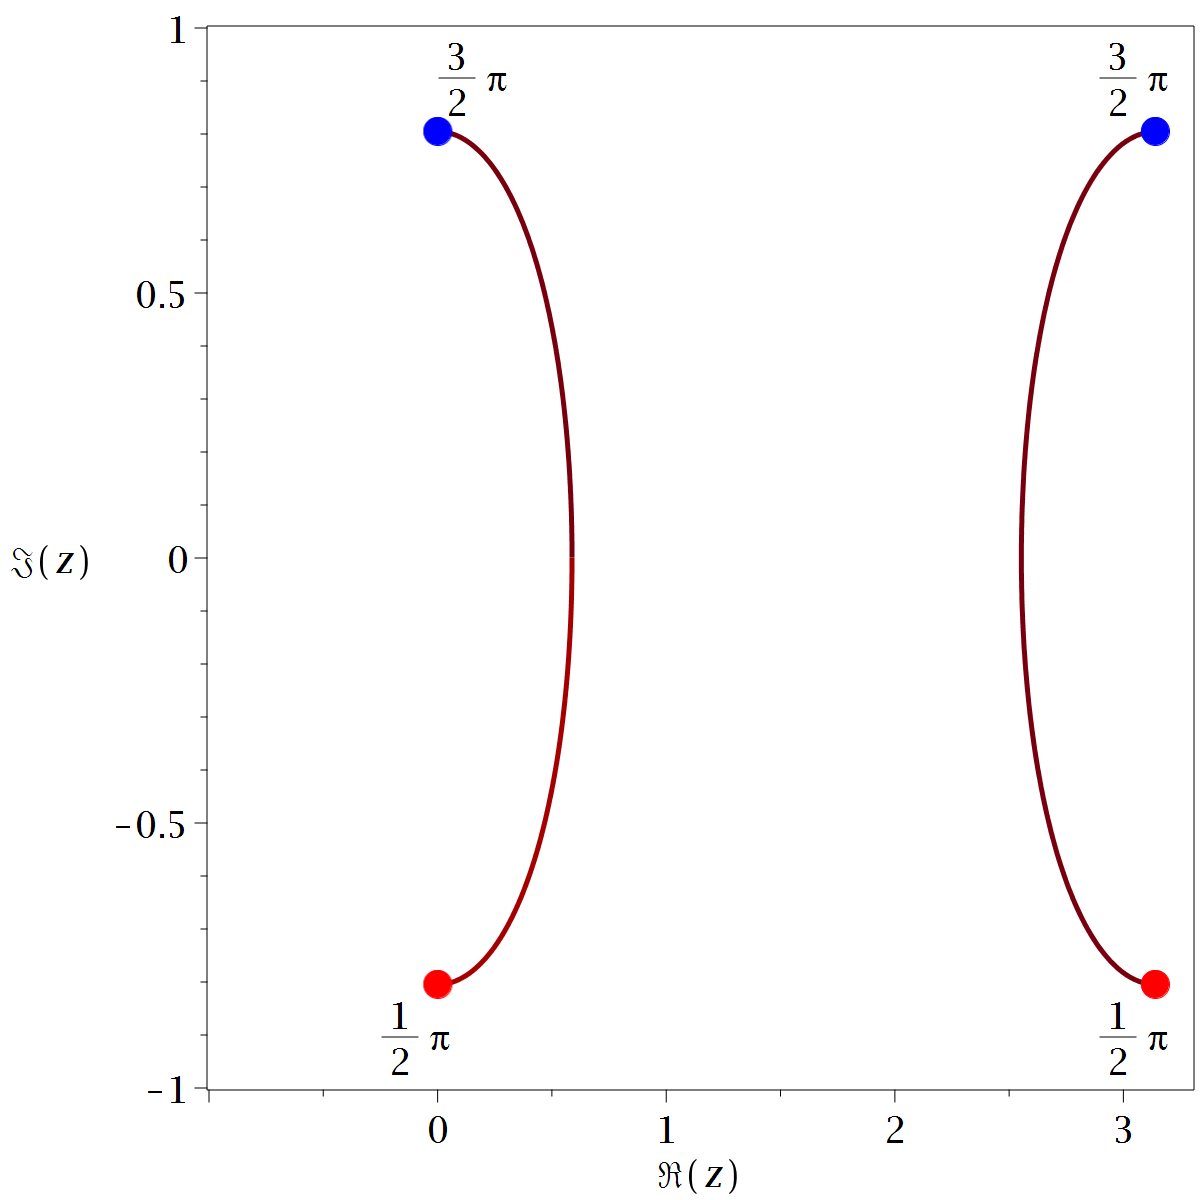
\includegraphics[width=0.45\textwidth]{acotJump.png}
        \label{fig:acotJump}%
    }
    \caption{Plots for the arccotangent function $\acot@{z}$ with $z = \frac{3}{2}\expe^{\iunit\phi}$, where $\phi \in [0,2\cpi]$. Figure~\protect\subref{fig:acotCont} illustrates a branch cut defined at $[-\iunit, \iunit]$ and figure~\protect\subref{fig:acotJump} illustrates the branch cuts defined at $(-\infty\iunit, -\iunit]$ and $[\iunit, \infty\iunit)$. The blue and red dots represents the positions, where the function jumps over the branch cuts in~\protect\subref{fig:acotJump}.}
    \label{fig:acot}
\end{figure}

We provide the following solution for such problems. Instead of translating the function itself, the translator uses other equivalent representations for the function. In case of the arccotangent function, we can use the following alternative representations, based on the suggestions in~\cite{Branches:acot}.

Note that the following notation uses our standard notation for a translation from semantic \LaTeX{} to \Maple. We will introduce this notation in a formal way later in section~\ref{sec:definition}.

\begin{eqnarray}
\verb|\acot@{z}| & \overset{\langMaple}{\mapsto} & \verb|arccot(z)|\label{eq:acot-alternatives}\\
& \overset{\langMaple}{\mapsto} & \verb|arctan(1/z)|\label{eq:acot-alternatives-1}\\
& \overset{\langMaple}{\mapsto} & \verb|I/2*ln((z-I)/(z+I))|\label{eq:acot-alternatives-2}
\end{eqnarray}

As illustrated above, translation~(\ref{eq:acot-alternatives}) contains the branch cut issue. Translation~(\ref{eq:acot-alternatives-1}) is an alternative, because the arctangent function in \Maple{} has the same position for the branch cut of the arctangent function in the \gls{dlmf}. However, in this case, the arccotangent function would be no longer defined at $z=0$. Translation~(\ref{eq:acot-alternatives-2}) is another alternative and defined at $z=0$. 

A more complicated example might be the equation of the already introduced parabolic cylinder function $\ParabolicU@{a}{z}$ and the modified Bessel function of the second kind $\BesselK{\nu}@{z}$. The parabolic cylinder function is a solution of a second order differential equation~\cite[(12.2i)]{NIST:DLMF} and can be represented by $\BesselK{\nu}@@{z}$ for $a=0$. The relation is defined in~(\ref{eq:branch-cut-issue}). 

\begin{equation}\label{eq:branch-cut-issue}
\displaystyle \ParabolicU@{0}{z} = \sqrt{\frac{z}{2\cpi}}\BesselK{\frac{1}{4}}@{\frac{1}{4}z^2}
\end{equation}

Following the same approach as for the arccotangent function discovers results in a branch cut problem. Figure~\ref{fig:u-bessel} illustrates that problem for equation~(\ref{eq:branch-cut-issue}) with $z=2.5\expe^{\iunit\phi}$ and letting $\phi$ increase from $0$ to $2\cpi$. While the left hand side is an entire function of $z$ (can be seen in figure~\ref{fig:u-cont}), the right hand side has two functions with a branch cut along the negative real axis each. As already discussed, the branch cut of the square root function is at $(-\infty,0]$. Therefore, at $\phi = \cpi$ the right hand side jumps over the branch cut (green dots) back to the principal branch rather than continue on the other branch. Furthermore, the principal branch of $K_\nu$ is defined for $\phi \in (-\cpi,\cpi]$. With $z^2 = r^2\expe^{2\iunit\phi}$, the branch cut of $K_\nu$ is reached at $\phi = \left\{ \frac{\cpi}{2}, \frac{3\cpi}{2} \right\}$ (red dots and blue dots). The branch cut of $K_\nu$ "moves" to $(-\infty\iunit,0]$ and $[0,\infty\iunit)$. Hence, we end up with three branch cuts for the right hand side of (\ref{eq:branch-cut-issue}).

\begin{figure}[!ht]
    \centering
    \subfloat[The left hand side of (\ref{eq:branch-cut-issue}).]{%
        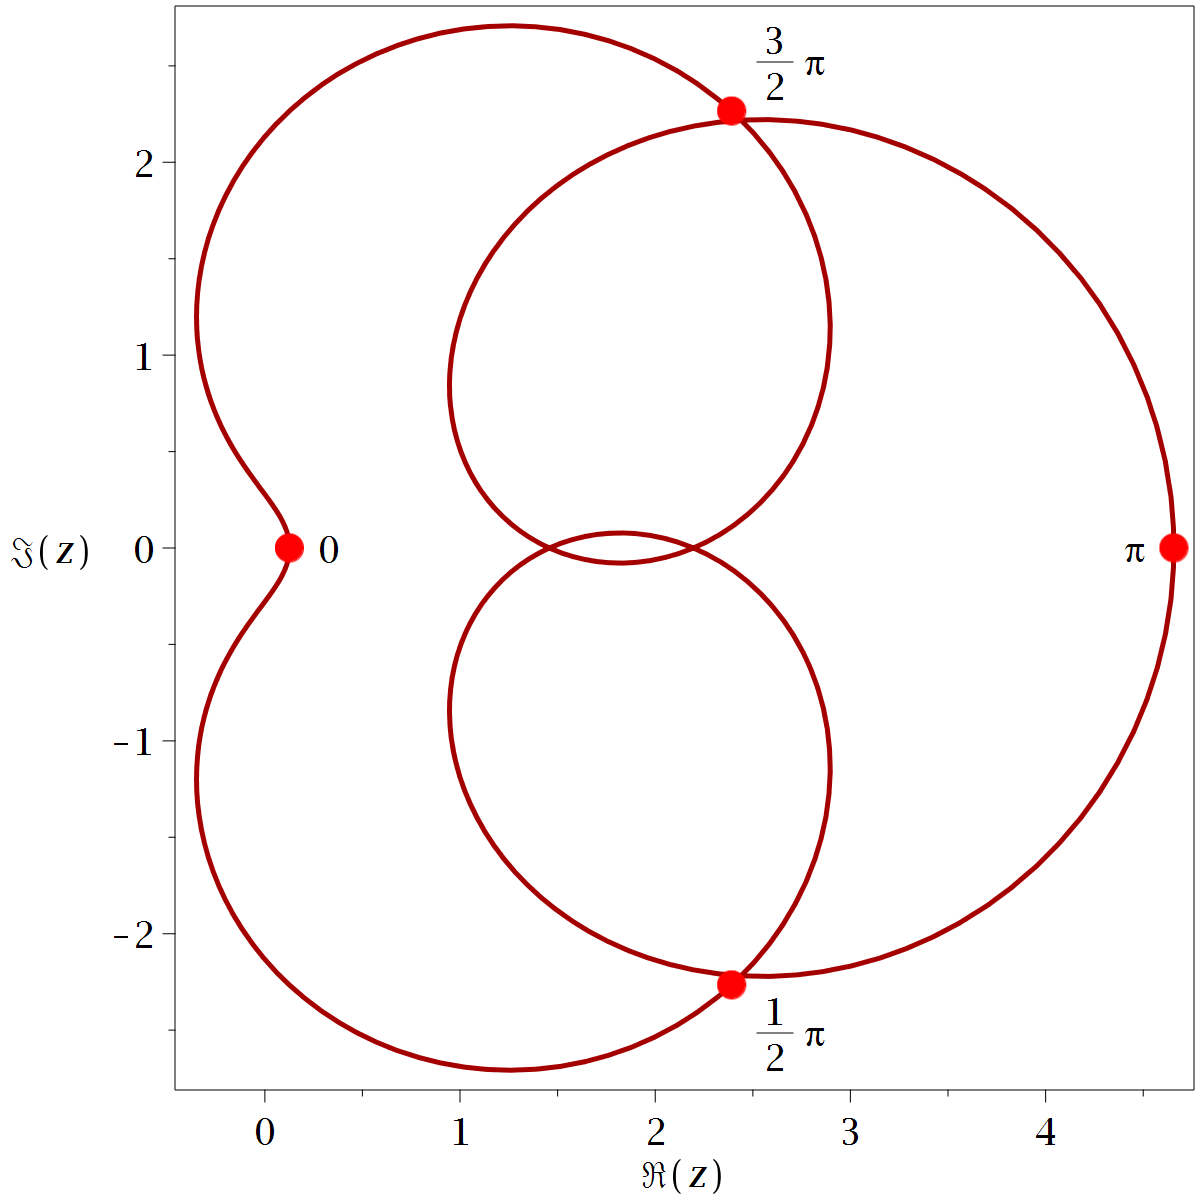
\includegraphics[width=0.45\textwidth]{CylinderU.png}
        \label{fig:u-cont}%
    }
    \hspace{1cm}
    \subfloat[The right hand side of (\ref{eq:branch-cut-issue}).]{%
        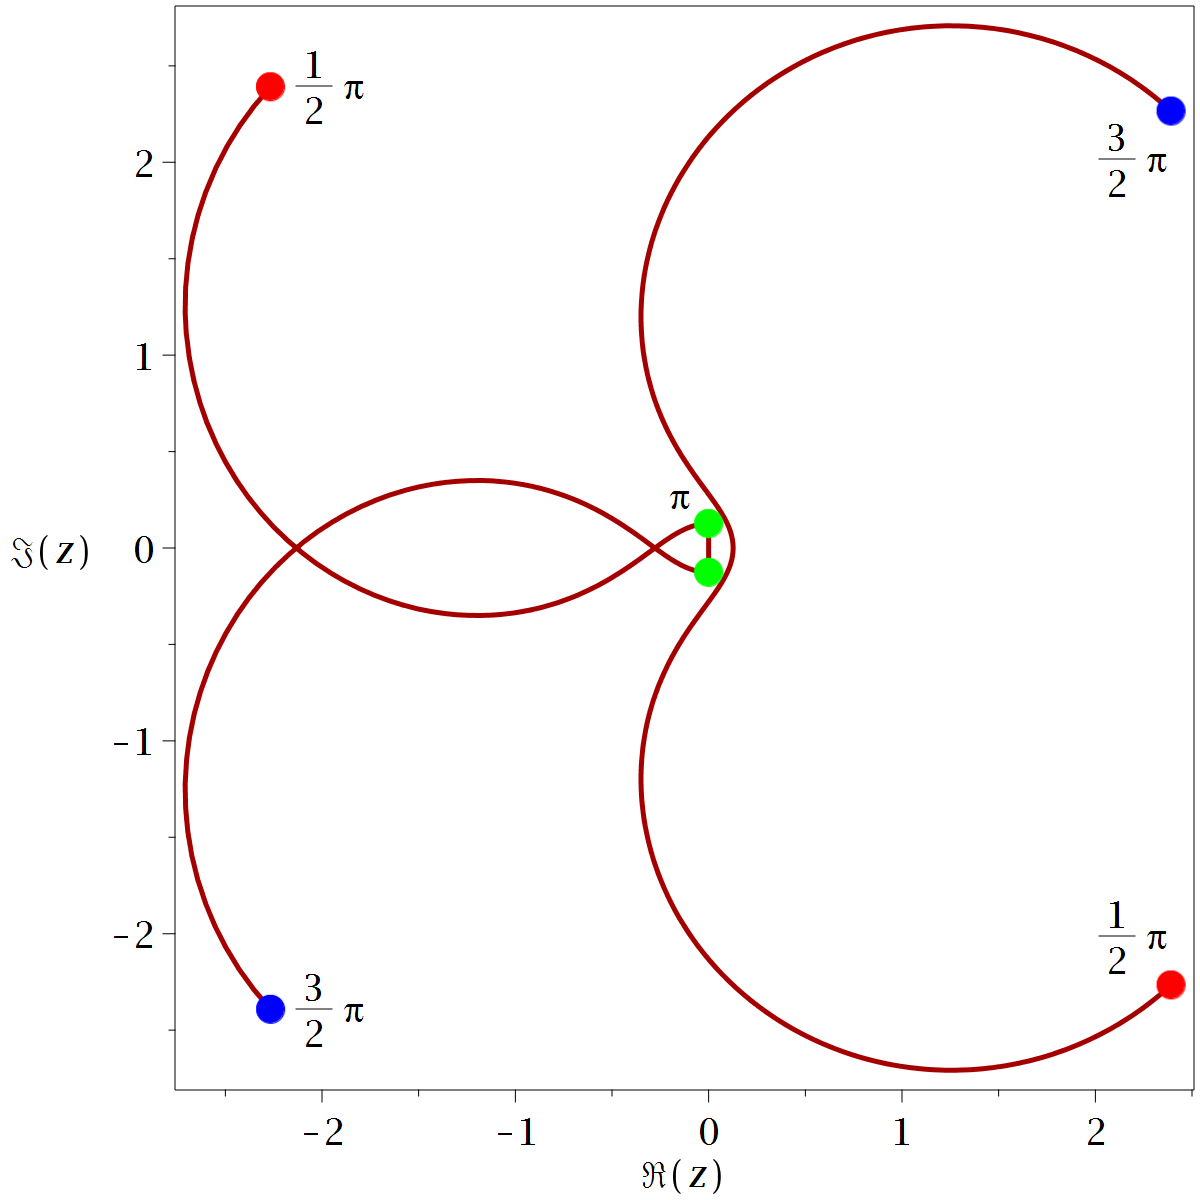
\includegraphics[width=0.45\textwidth]{WithCuts.png}
        \label{fig:bessel-cut}%
    }
    \caption{Two polar plots with $z=2.5\expe^{\iunit\phi}$ for $\phi \in [0,2\cpi]$ of left and right hand side of (\ref{eq:branch-cut-issue}) in \Maple. $U$ is an entire function, while $K_\nu$ and the square root function have a branch cut along $(-\infty,0]$. The colored dots represent the jumps over the branch cuts.}
    \label{fig:u-bessel}
\end{figure}

Since \gls{cas} do not provide Riemann surfaces, we use another approach to solve this problem, called \textbf{analytic continuation}. Analytic continuation is the process of extending the range of validity of a representation or more generally extending the region of definition of an analytic function~\cite[152]{ComplexVariables}. For the modified Bessel function of the second kind the analytic continuation is defined in the \gls{dlmf}~\cite[(10.34.4)]{NIST:DLMF}. With analytic continuation, the right hand side of equation~(\ref{eq:branch-cut-issue}) is illustrated in figure~\ref{fig:analytic-cont}.

\begin{figure}[!ht]
    \centering
    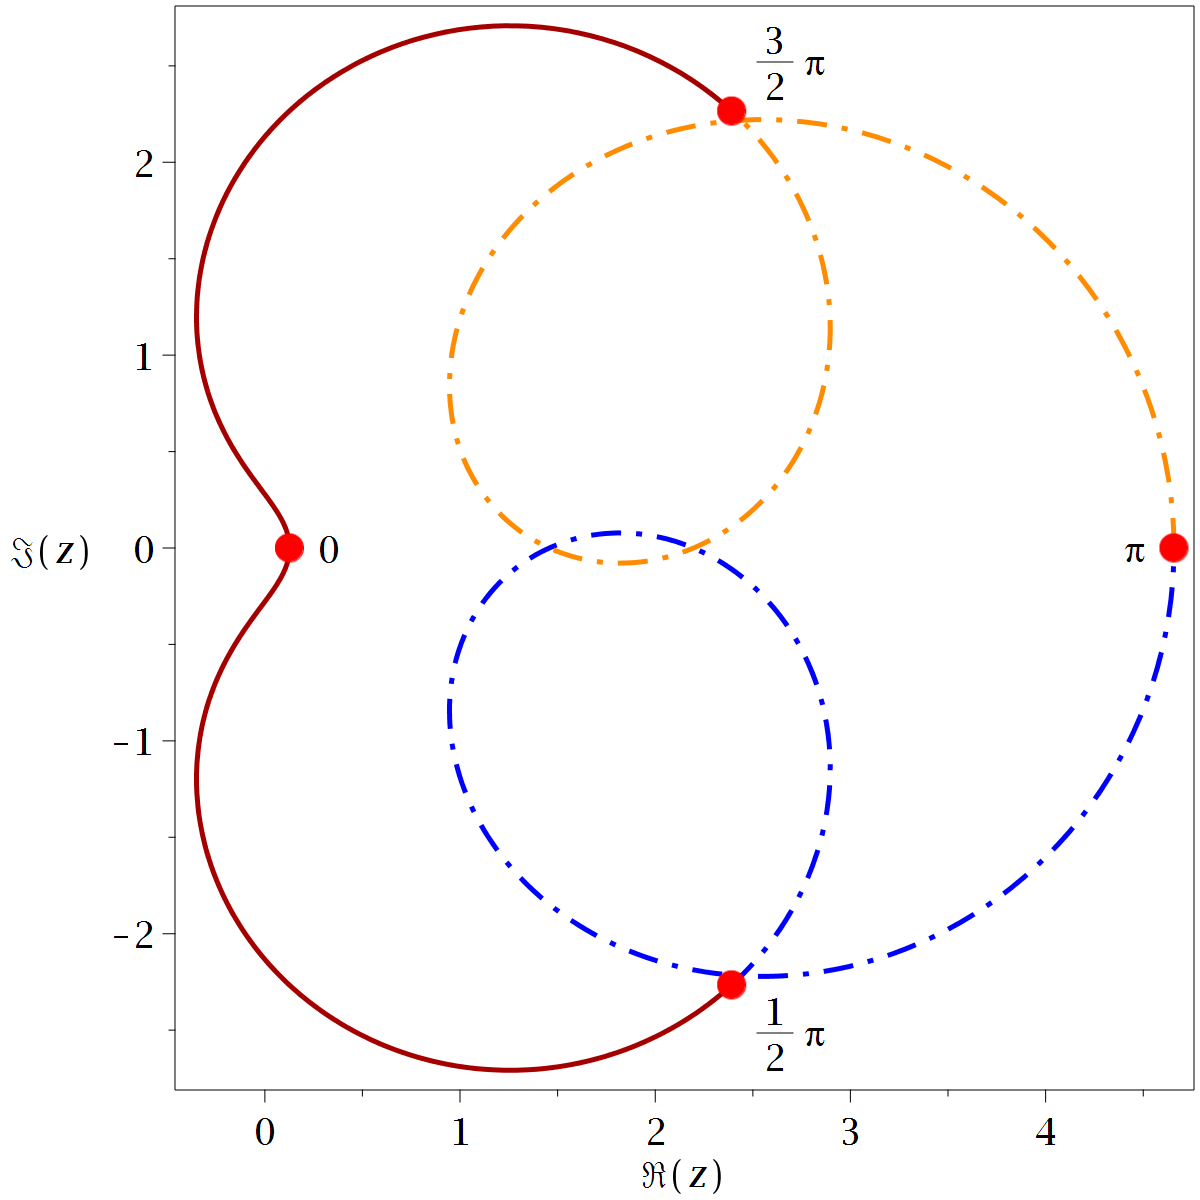
\includegraphics[width=0.6\textwidth]{WithAnalyticCont.png}
    \caption{The right hand side of (\ref{eq:branch-cut-issue}) using analytic continuation, when the function jumps over the branch cut at $\phi = \left\{\frac{\cpi}{2},\cpi\right\}$. At $\phi = \frac{3\cpi}{2}$, the function jumps back to the principal branch.}
    \label{fig:analytic-cont}
\end{figure}

\subsection{Injective, Surjective \& Bijective Mappings}
Later in the thesis, we will define our translation as a function. Since our main goal is to provide bijectivity for our translation, we will briefly introduce the terminology.

Consider a function $f: X \mapsto Y$.

\begin{definition}[Injective Function]
The function $f$ is \textbf{injective} if
\begin{equation}
\forall x,x' \in X: \quad f(x) = f(x') \Rightarrow x = x'.
\end{equation}
\end{definition}

\begin{definition}[Surjective Function]
The function $f$ is \textbf{surjective} if
\begin{equation}
\forall y \in Y, \exists x \in X: \quad y = f(x).
\end{equation}
\end{definition}

\begin{definition}[Bijection]
The function $f$ is \textbf{bijective} if $f$ is injective and surjective.
\end{definition}

The most useful part about bijective mappings is that every bijective function $f$ has an inverse function $f^{-1}$. Consider a translation between two systems as a function that is bijective. Such a translation has an inverse function, or in other words backward translation. This would allow us to translate each expression in one system to the other and back again.

Obviously, such a translation is desirable. However, we will see that this goal is not achievable for all possible expressions. Even worse, we will see that our translation is neither injective nor surjective.

\subsection{Graphs and Trees}
\glsreset{dag}
A typical way to formalize the structure of mathematical expressions are trees. We will briefly introduce what trees are and what an expression tree is.

\begin{definition}[Graph]
A \textbf{graph} is an ordered pair $G=(V,E)$, where $V$ is the set of \textbf{vertices} (or \textbf{nodes}) and $E$ the set of \textbf{edges}, which are a 2-element subset of $V$.
\end{definition}

\begin{definition}[Directed Graph]
A \textbf{directed graph} (sometimes also referred as \textbf{digraph}) $G = (V,E)$ is a graph with oriented edges. That means $E$ is a set of ordered pairs of vertices. Therefore, a graph is \textbf{undirected} if all edges $e \in E$ have no orientation.
\end{definition}

\begin{definition}[Paths, Cycles and connected Graphs]
Let $G = (V,E)$ be a directed or undirected graph with at least three vertices ($|V| \geq 3$). A \textbf{path} from one vertex $i\in V$ to another $j\in V$ is a finite sequence of vertices and edges
\begin{equation}
i = i_1, (i_1, i_2), i_2, \ldots , i_{k-1}, (i_{k-1}, i_k), i_k = j.
\end{equation}
A path is a \textbf{cycle} if $i = j$. If a graph $G = (V,E)$ has no cycles, it is called \textbf{acyclic}. Furthermore, if there is a path for every pair of vertices, $G$ is called \textbf{connected}.
\end{definition}

A \gls{dag}, for example, is used internally to represent mathematical expressions. However, another way to represent mathematical expressions are trees.

\begin{definition}[Tree]
A \textbf{tree} $T = (V,E)$ is an acyclic and connected graph.
\end{definition}

Let $T = (V,E)$ be a tree and $r \in V$. We call $r$ \textbf{root} of $T$ and order the other nodes in an ascending ordering according to its length of the path to $r$. Each node $v \in V$, which is directly connected with $r$ is called \textit{child} of $r$ and $r$ is called \textit{parent} of $v$. This can be defined for all nodes in the tree which created a hierarchical structure in the tree. A node is in a higher hierarchy, when it is closer to root node. A node can have multiple \textit{children}. Consider a node $a \in V$ as a node with three children $u,v,w$. We also define a order for the children, so that $u < v < w$. \textbf{Siblings} are nodes that share the same parent node. With the order we call $u$ the previous sibling of $v$ and $w$ the following sibling of $v$. With this additional terminology, we can move through trees easily. Trees with an ordering for all nodes and a root node are also called \textbf{ordered trees}.

Mathematical expressions can be represented by ordered trees consisting of terminal symbols, such as identifiers or numbers (leaf nodes), and functions or operators (non-leaf nodes)~\cite{VMEXT}. Consider the mathematical expression
\begin{equation}\label{eq:simple-expr}
\expe^{x} + \frac{x^2}{\cpi}.
\end{equation}

The tool \gls{vmext}~\cite{VMEXT} visualizes expression trees. Figure~\ref{fig:simple-expr-tree} draws the expression tree for (\ref{eq:simple-expr}).

\begin{figure}[ht]
    \centering
    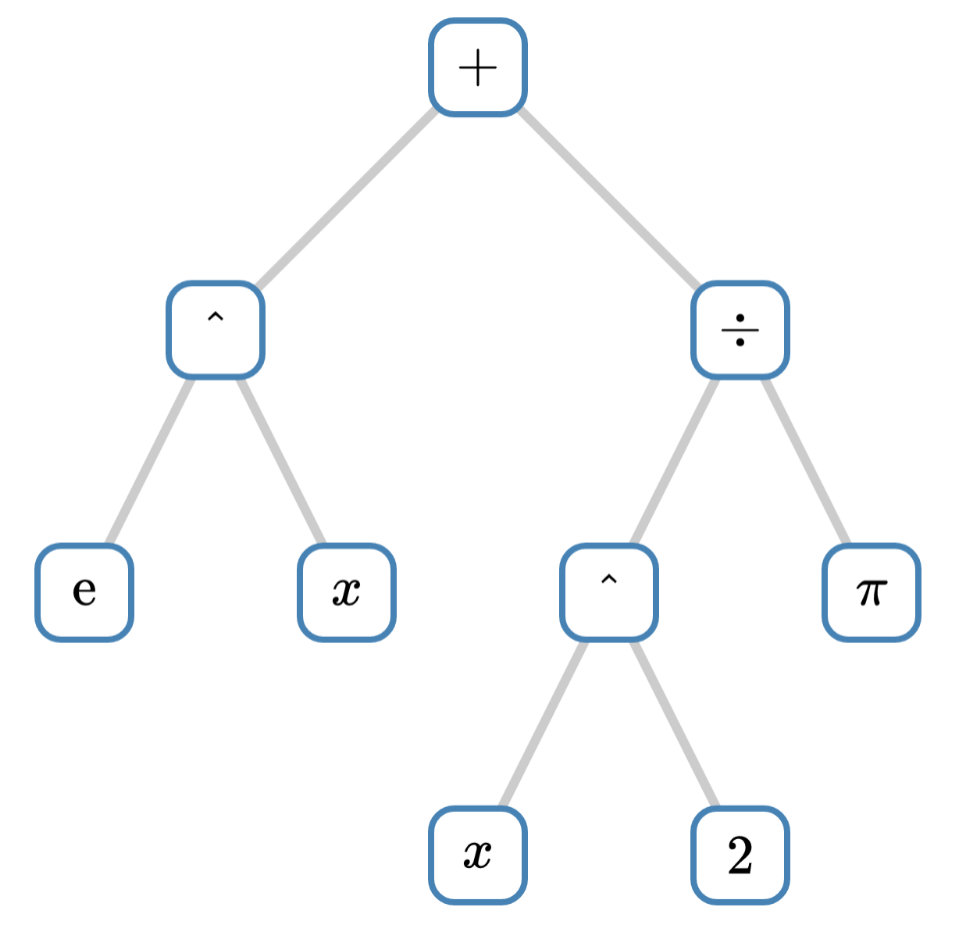
\includegraphics[width=0.7\textwidth]{expressionTreeSimple.png}
    \caption{The expression tree of (\ref{eq:simple-expr}) visualized with VMEXT~\cite{VMEXT}.}
    \label{fig:simple-expr-tree}
\end{figure}